\documentclass[tikz,border=2pt]{standalone}
\usepackage{amsmath}
\usetikzlibrary{arrows.meta,decorations.pathreplacing}
\begin{document}
% Apply(s, x -> 1{x > 3}) on the service times s = [1, 2, 4, 5] gives [0, 0, 1, 1];
% Sum([0, 0, 1, 1]) / 4 = 1/2 is the fraction of long services (Section 1.2).
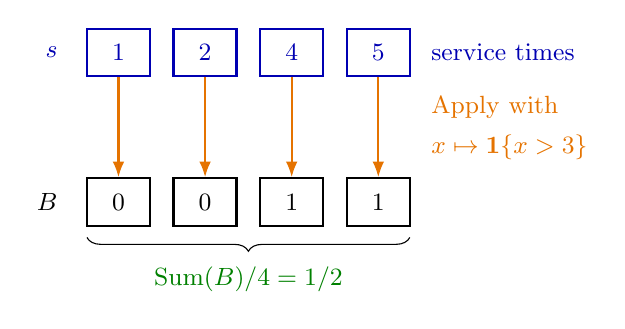
\begin{tikzpicture}[font=\small, >={Latex[length=2mm]},
  cell/.style={draw, thick, minimum width=0.8cm, minimum height=0.6cm}]
  \foreach \v/\b [count=\i] in {1/0,2/0,4/1,5/1} {
    \node[cell, blue!70!black] (s\i) at (1.1*\i,1.9) {$\v$};
    \node[cell, black] (b\i) at (1.1*\i,0) {$\b$};
    \draw[->, orange!90!black, thick] (s\i.south) -- (b\i.north);
  }
  \node[blue!70!black, anchor=east] at (0.45,1.9) {$s$};
  \node[anchor=east] at (0.45,0) {$B$};
  \node[orange!90!black, anchor=west] at (4.95,1.2) {$\operatorname{Apply}$ with};
  \node[orange!90!black, anchor=west] at (4.95,0.7) {$x\mapsto\mathbf{1}\{x>3\}$};
  \node[blue!70!black, anchor=west] at (4.95,1.9) {service times};
  \draw[decorate, decoration={brace, mirror, amplitude=5pt}] (0.7,-0.45) -- (4.8,-0.45);
  \node[green!50!black, anchor=north] at (2.75,-0.7) {$\operatorname{Sum}(B)/4=1/2$};
\end{tikzpicture}
\end{document}
